\documentclass[11pt]{article}
\usepackage{../cs70, latexsym,epsf,amsmath,amsfonts,graphicx,url}

\lecture{7}
\def\title{Note \the\lecturenumber}

\newcounter{thm}
\addtocounter{thm}{\the\lecturenumber}


\newtheorem{theorem}{Theorem}[thm]
\newtheorem{algorithm}{Algorithm}[thm]
\newtheorem{lemma}{Lemma}[thm]
\newtheorem{fact}{Fact}[thm]
\newtheorem{definition}{Definition}[thm]
\newtheorem{conjecture}{Conjecture}[thm]
\newtheorem{counterexample}{Counterexample}[thm]
\newtheorem{corollary}{Corollary}[thm]
\newtheorem{observation}{Observation}[thm]

%%% Alistair's Macros
\makeatletter
\def\eqalign#1{\,\vcenter{\openup\jot\m@th
  \ialign{\strut\hfil${##}$&${{}##}$\hfil
      \crcr#1\crcr}}\,}
\def\eqalignno#1{\displ@y \tabskip\@centering
  \halign to\displaywidth{\hfil${##}$\tabskip\z@skip
    &${{}##}$\hfil\tabskip\@centering
    &\llap{$##$}\tabskip\z@skip\crcr
    #1\crcr}}
\makeatother
%%% End Alistair's Macros

\begin{document}
\maketitle

\iffalse
{\it This note is partly based on Section~1.4 of ``Algorithms," by S.~Dasgupta, C.~Papadimitriou
and U.~Vazirani, McGraw-Hill, 2007. \\An online draft of the book is available at
http://www.cs.berkeley.edu/~vazirani/algorithms.html}
\fi

\section{Bijections}\label{scn:bijection}

The notion of a mathematical \emph{function}, i.e. a mapping $f$ from an input set $A$ to an output set $B$, is ubiquitous in our everyday lives. For example, your professor might assign you a letter grade of $A$ through $F$ based on a function which maps your numerical grade, i.e. an integer from $0$ to $100$, to the set $\set{``A",``B",``C",``D",``F"}$. Or consider the process of paying federal taxes, in which your income level in dollars is mapped via a function to a tax bracket which dictates the percentage of tax you must pay. Both of these are examples of {functions}, which most generally can be described using the notation $f:A\mapsto B$. Here, $A$ is a set called the \emph{domain} of $f$, and $B$ is a set known as the \emph{range} of $f$. Of all the possible functions in the wild, there is a special type which turns out to be particularly useful in computer science, specifically in the study of cryptography --- namely, the notion of a \emph{bijective} function. It is this class of functions which we study in this lecture.

\sanity{Consider the ``birthday function'' $f$, which given a person's birth date, outputs the age of that person. What are the domain $A$ and range $B$ of $f$?}

Intuitively, a \emph{bijection} is a function with the property that any output of the function can be uniquely mapped back to some input. More formally, a function $f:A\mapsto B$ is a bijection iff for all $b\in B$, there exists a unique \emph{pre-image} $a\in A$ such that $f(a)=b$. Let us demonstrate with the following example of a function $f:\set{0,\ldots,m-1}\mapsto\set{0,\ldots,m-1}$:
$$
f(x) = x + 1 \bmod m.
$$
Here, $f$ is a bijection since the unique pre-image of any $y\in \set{0,\ldots,m-1}$ is $y - 1$. The special case of $m=4$ is depicted in Figure~\ref{fig:bij1}; note the special property that each element on the right side has precisely one matching element on the left side.
\begin{figure}[h]
\begin{center}
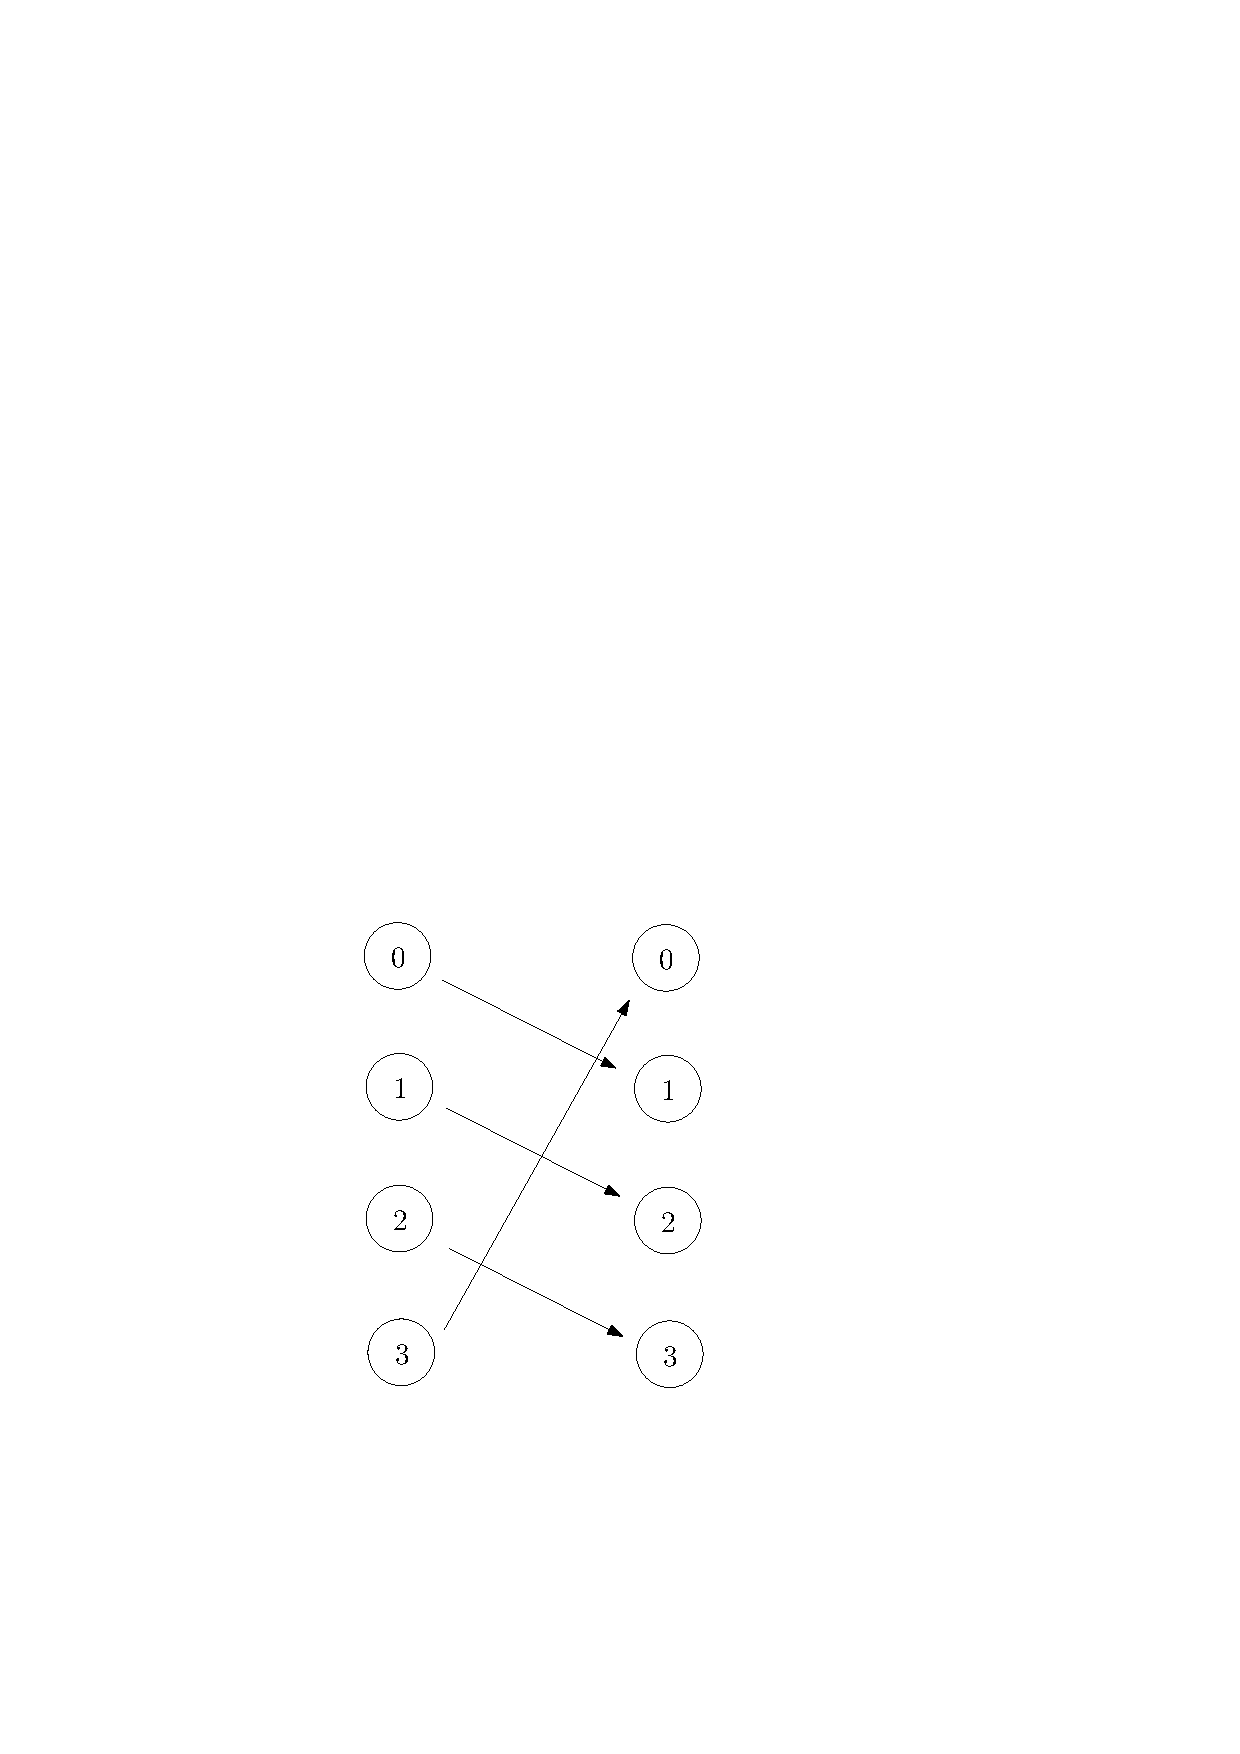
\includegraphics[scale=0.55]{bij1.pdf}
\end{center}
\caption{The bijection $f(x) = x + 1 \bmod 4$ with domain $A=\set{0,\ldots,3}$ and range $B=\set{0,\ldots,3}$.}
\label{fig:bij1}
\end{figure}

\pagebreak

\sanity{Consider the same function $f(x) = x + 1 \bmod 4$, except now with $A=\set{0,\ldots,4}$ and range $B=\set{0,\ldots,3}$. Is $f$ still a bijection? Why not? (Give two elements of $A$ which map to the same element of $B$.)}

If you stare at Figure~\ref{fig:bij1} long enough, you might realize that the property of being a bijection is actually equivalent to having two separate properties: (1) Each element on the right has \emph{some} pre-image on the left, and (2) if two arrows are incident on an element on the right, then both arrows must originate from the same element on the left. More formally, these properties can be stated as:
\begin{enumerate}
\item $f$ is {\em onto} or \emph{surjective}: Any $b \in B$ has a pre-image in $A$, i.e. for all $b\in B$ there exists an $a\in A$ such that $f(a)=b$.
\item $f$ is {\em one-to-one} or \emph{injective}: For all $a,a'\in A$, if $f(a) = f(a')$ then $a = a'$.
\end{enumerate}

To help solidify our understanding of bijections, let us consider two more functions. First, recall the example given at the start of this lecture about the function mapping a numerical grade in the set $\set{0,1,\ldots,100}$ to a letter grade $\set{``A", ``B", ``C", ``D", ``F"}$. Is this a bijection?
\emph{No}, since each letter grade has many numerical grades mapped to it. (In fact, it is worth noting that there \emph{cannot} exist a bijection between these two sets, since they have different sizes. This connection between bijections and set sizes is the key to Cantor's celebrated idea that there is more than one notion of infinity!) Next, consider the following function $g$ mapping $\{0,\dots,m-1\}$ to itself:
\begin{equation}\label{eqn:1}
g(x) = 2x \bmod m.
\end{equation}
It turns out that $g$ is only a bijection if $m$ is odd.

\sanity{
\begin{enumerate}
\vspace{-2mm}
	\item Show that for the value $m=4$, the function $g$ is not a bijection since it is not one-to-one. Can you generalize your proof to arbitrary $m$?
	\item Draw a diagram analogous to Figure~\ref{fig:bij1} to show that for $m=5$, the function $g$ is a bijection.
	\vspace{-2mm}
\end{enumerate}
}

A nice alternate way of thinking about bijectivity is the following, which will prove useful in our discussion on cryptography in this lecture.

\begin{lemma}\label{l:inverse}
A function $f: A\rightarrow A$ is a bijection iff there is an {\it inverse\/} function $g: A\rightarrow A$ such that $g(f(x)) = x$ and $f(g(y)) = y$ for all $x,y \in A$.
\end{lemma}
\begin{proof}
We give a direct proof. First assume there exists an inverse function $g$ as described in the claim. Then, to see that $f$ is one-to-one, note that whenever $f(x) = f(x')$, we have that $x = g(f(x)) = g(f(x')) = x'$, as desired. To see that $f$ is onto, note that for any $y \in A$ we have $f(g(y)) = y$, so $g(y) \in A$ is the pre-image of $y$.

Conversely, assume $f$ is bijective. This means every $y \in A$ has a unique pre-image $x \in A$ such that $f(x) = y$. Define $g \colon A \to A$ by $g(y) = x$. Then we see that by construction, we have $f(g(y)) = y$, and similarly, $g(f(x)) = g(y) = x$. This shows that $g$ is the inverse function of $f$, as desired.
\end{proof}

\pagebreak
\sanity{Show that the function $g$ from Equation~(\ref{eqn:1}) is a bijection for the case $m=5$ by explicitly describing an inverse function as in Lemma~\ref{l:inverse}.}


\section{Fermat's Little Theorem}

In 1640, Pierre de Fermat stated one of the fundamental results of elementary number theory, nowadays known as \emph{Fermat's Little Theorem}. Ultimately, our goal in this lecture is to study the use of bijections in cryptography, and it turns out Fermat's Little Theorem will be a crucial tool in this venture. Thus, we state and prove it now. Its proof also uses the concept of a bijection.

\begin{theorem}\label{fermat} {\bf [Fermat's Little Theorem]} For any prime~$p$
and any $a\in\{1,2,\ldots,p-1\}$, we have $a^{p-1}\equiv1\bmod p$.
\end{theorem}
\begin{proof}
Let $S = \{1,2,\ldots, p-1\}$. We give a direct proof consisting of two parts. First, we show that the function $f: S\rightarrow S$ such that $f(x) \equiv ax\bmod p$ is a bijection. Second, we use the fact that $f$ is a bijection to prove the claim.

\sanity{
Verify that for $a = 3, p = 7$, the function $f(x) \equiv ax\bmod p$ is a bijection corresponding to the image below.

\begin{figure}[h]
\begin{center}
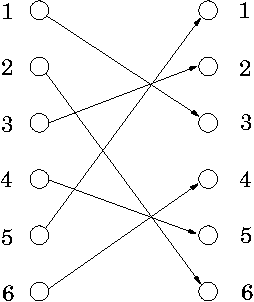
\includegraphics[scale=0.8]{bij.pdf}
\end{center}
\caption{Multiplication by (3 mod 7)}
\label{fig:bij}
\end{figure}
}
\noindent

To prove that $f$ is indeed a bijection, since the domain and range of $f$ are the same set $S$, it suffices to prove that $ax\bmod p$ and $ax'\bmod p$ are distinct if $x\neq x'$. To prove the latter, assume for sake of contradiction that there exist distinct $x,x'\in S$ such that
\[
	a \cdot x \equiv a \cdot x' \pmod p.
\]
Then, since by definition $a$ is non-zero, and since $a$ and $p$ are co-prime, then by Theorem~6.2,
 we know $a$ has a multiplicative inverse $a^{-1}$ modulo $p$. Multiplying both sides of the equation above by $a^{-1}$ thus yields $x \equiv x' \pmod p$, which contradicts our assumption that $x$ and $x'$ are distinct. We conclude that $f$ is a bijection.

Let us now prove our main claim. Since $f$ is a bijection, its image is $S$; this implies that
the product of all elements in $S$ equals the product of all elements in the image of $f$. Specifically, we have
\[
	(p-1)! \equiv a^{p-1} \cdot (p-1)! \pmod p.
\]
Since $(p-1)!$ is relatively prime to $p$, it again follows by Theorem~6.2
that we can divide both sides of this equation by $(p-1)!$, yielding the desired statement.
\end{proof}


\section{Public Key Encryption and RSA}

One of the oldest and most fundamental problems facing mankind has been: How to send a message securely from a sender, say Alice, to a receiver Bob, so that an eavesdropper Eve gains little to no information about the message? As you might imagine, this task has a host of applications in areas ranging from banking to the military. In fact, Julius Caesar himself was known to use an encryption scheme nowadays known as the \emph{Caesar cipher} in order to protect messages of military significance. Unfortunately, Caesar's cipher had a significant drawback: In order to encode and decode messages, one needed to know a \emph{secret key}. This led to a chicken-and-the-egg scenario --- how does Alice share her secret key with Bob without Eve learning anything about it to begin with? In the 1970s, a breakthrough solution to this problem was discovered in the form of \emph{public key encryption}.

In public key encryption, there are \emph{two} keys: One for encryption, $E$, which is public knowledge to everyone, and one for decryption, $D$, which is known only by the receiver, Bob. In this way, \emph{anyone in the world} can send Bob a secret message: The sender encodes the message using $E$, sends the encrypted message to Bob, who then decrypts it using $D$. How could such a scheme be possible? It turns out the secret ingredient is a special bijection which is easy to compute (i.e. anyone in the world can do it), but believed to be very difficult to \emph{invert} without knowledge of a secret key, which only Bob possesses. This special bijection is known as the RSA function, named after its inventors Ronald Rivest, Adi Shamir and Leonard Adleman, and is as follows:
\[
E(x) \equiv x^e \bmod N,
\]
where $N= pq$ for two large primes $p$ and $q$, $E: \{0,\dots,N-1\}\mapsto\{0,\dots,N-1\}$,
and $e$ is relatively prime to $(p-1)(q-1)$. It may not be clear \emph{a priori} that this is indeed a bijection; we shall prove this shortly. The inverse of the RSA function is given by the decryption operation:
\[
	D(x) \equiv x^d \bmod N
\]
where $d$ is the multiplicative inverse of $e\bmod (p-1)(q-1)$. RSA now works as follows: The public key is $(N,e)$, known to everyone in the world, and the private key is $d$, known only to Bob. To send a secret message $x\in\set{1,\ldots,N-1}$ to Bob, Alice applies the {\it encryption function}~$E$ to~$x$ to obtain a {\it ciphertext} $E(x)$, which she then sends to Bob. Upon receipt of Alice's ciphertext~$E(x)$, Bob applies his {\it decryption function\/}~$D$ to recover $x$. This should convince you that RSA allows you to indeed encrypt and decrypt a message $x$. But is it \emph{secure}? We defer this discussion to Section~\ref{sscn:security}. For now, let us prove that indeed $D(E(x)) = x$ for all $x\in\set{1,\ldots, N-1}$, which in turn (by Theorem~\ref{l:inverse}) implies that $E$ is a bijection.

\begin{theorem}\label{thm:1}
For $E$ and $D$ as defined above, we have $D(E(x)) = x\bmod N$ for all $x\in\{0,1,\ldots,N-1\}$.
\end{theorem}
\begin{proof} To prove the statement, we have to show
that
\begin{equation}\label{eqn:1}
(x^e)^d = x\bmod N\qquad\hbox{\rm for every $x\in\{0,1,\ldots,N-1\}$},
\end{equation}
where recall $N= pq$ for primes $p$ and $q$, $\gcd(e,(p-1)(q-1))=1$, and $d$ is the multiplicative inverse of $e\bmod (p-1)(q-1)$. Let's consider the exponent, which is~$ed$.  By definition of~$d$, we know that
$ed=1\bmod (p-1)(q-1)$; hence we can write $ed = 1+k(p-1)(q-1)$ for some integer~$k$,
and therefore
\begin{equation}\label{eqn:2}
  x^{ed} - x = x^{1+k(p-1)(q-1)} - x = x(x^{k(p-1)(q-1)}-1).
\end{equation}
Looking back at Equation~(\ref{eqn:1}), our goal is to show that this last expression
in Equation~(\ref{eqn:2}) is equal to~0 mod~$N$ for every~$x$. To do this, we show that the expression is divisible both by $p$ and $q$; thus, since $p$ and $q$ are primes, the expression must also be divisible by $N=pq$, which will yield our claim.

We begin by showing that $x(x^{k(p-1)(q-1)}-1)$ in~(\ref{eqn:2}) is divisible by~$p$.  We have two cases to consider:
\begin{itemize}
\item[{\bf Case 1:}]  ({\it $x$ is a multiple of~$p$}) In this case, $p$ clearly divides the expression in~(\ref{eqn:2}) since $p\mid x$.
\item[{\bf Case 2:}] ({\it $x$ is not a multiple of~$p$}) Since $x\ne 0\bmod p$,
we can use Fermat's Little Theorem to deduce that $x^{p-1}=1\bmod p$. Then $(x^{p-1})^{k(q-1)}\equiv 1^{k(q-1)}\bmod p$, which implies that $x^{k(p-1)(q-1)}-1=0\bmod p$, and so $p$ divides the expression in~(\ref{eqn:2}).
\end{itemize}
The proof that $q\mid x(x^{k(p-1)(q-1)}-1)$ is identical. This completes the proof.
\end{proof}

\subsection{Security of RSA}\label{sscn:security}

We have thus far shown that the RSA protocol is {\it correct}, in the sense that Alice can encrypt messages in such a way that Bob can reliably decrypt them again.  But how do we know that it is {\it secure}, i.e., that Eve cannot obtain any information about Alice's message $x$ from the ciphertext $E(x)$? To be clear, there is no known formal proof of this fact. Rather, the security of RSA hinges upon the following widely held \emph{assumption}:
\[
\hbox{\rm Given $N$, $e$ and $y=x^e\bmod N$, there is no efficient algorithm for
determining~$x$.}
\]
To help us appreciate why this assumption may be true, let us brainstorm how Eve might try to guess $x$: 
\begin{itemize}
    \item (Brute force) The naive approach would be via brute force --- simply try all possible values of $x$, each time checking whether $x^e=y\bmod N$. But this approach is unbelievably inefficient; Eve would have to try $O(N)$ values of $x$, which if $N$ is a $512$-bit number, boils down to $2^{512}$ values of $x$ to try --- this number is larger than estimates for the age of the Universe in femtoseconds!       
    \item (Reduction to factoring) Eve could be more clever and instead attempt to factor~$N$ to into its prime factors $p$ and~$q$; then, she could compute $d$ by determining the multiplicative inverse of~$e$ mod~$(p-1)(q-1)$. But this requires the ability to factor large numbers, a task which is \emph{also} considered impossible to solve efficiently.
        
    \item (Computing $(p-1)(q-1)$ directly) Finally, Eve could try to compute  $(p-1)(q-1)$ without factoring $N$; but it turns out this is equivalent to factoring $N$.
\end{itemize}

Thus, the hardness of RSA depends on the presumed difficulty of factoring large numbers, known as the \emph{Factoring Problem}. In fact, the Factoring Problem occupies a special place in theoretical computer science. It is one of the few known problems which is neither known to be efficiently solvable (i.e. in the complexity class P), nor intractable (i.e. complete for the class NP). However, there \emph{has} been a remarkable development over the last two decades; it turns out the Factoring Problem can be solved efficiently on a \emph{quantum} computer!

\sanity{Our discussion regarding the brute force approach above deserves a moment's reflection, in particular with respect to the following common fallacy: Namely, in order to try all possible factors $x$ of $N$ requires $O(N)$ iterations, which is often interpreted as ``polynomial time'' since the algorithm runs in time linear in $N$. Why is this algorithm \emph{not} ``polynomial time''? (Hint: What is the relevant quantity with respect to which we typically measure complexity?)}

\subsection{Implementations of RSA}

We close this note with a brief discussion of implementation issues regarding RSA.  Since we have argued that breaking RSA is impossible because {\it factoring\/} would take a very
long time, we should check that the computations that Alice and Bob themselves have
to perform are much simpler, and can be done efficiently.

There are really only two non-trivial things that Alice and Bob have to do:
\begin{enumerate}
\item Bob has to find prime numbers $p$ and~$q$, each having many (say, $512$) bits.
\item Both Alice and Bob have to compute exponentials mod~$N$.  (Alice has to
compute $x^e\bmod N$, and Bob has to compute $y^d\bmod N$.)
\end{enumerate}

Both of these tasks can be carried out efficiently. The first requires the implementation of an efficient test for primality as well as a rich source of primes. You will learn how
to tackle each of these tasks in the algorithms course CS170. The second requires
an efficient algorithm for modular exponentiation known as ``repeated squaring", which is not very difficult, but will also be discussed in detail in CS170.


To summarize, then, in the RSA protocol Bob need only perform simple calculations
such as multiplication, exponentiation and primality testing to determine the encryption and decryption keys. Similarly, Alice and Bob need only perform simple calculations to lock and
unlock the secret message respectively --- operations that any pocket computing device
could handle.  By contrast, to unlock the message without the key, Eve would have
to perform operations like factoring large numbers, which (at least according to widely
accepted belief) requires more computational power than all of the world's most sophisticated
computers combined!  This compelling guarantee of security without the need for
private keys explains why the RSA cryptosystem is such a revolutionary development
in cryptography.

\end{document}


